\subsection{Debayering}
Debayering is the process of estimating complete color information for an image that has been captured through a \gls{cfa}, particularly on the Bayer pattern \cite{getreuerMalvarHeCutlerLinearImage2011}.
In the Bayer pattern, green pixels cover half the array in a quincunx lattice, and the red and blue pixel locations are spaced uniformly every two pixels \cite{getreuerMalvarHeCutlerLinearImage2011}

Debayering is a type of demosaicking that involves interpolating the missing color information from the \gls{cfa} data.
Malvar, He, and Cutler proposed a simple linear method using 5 x 5 filters that shows surprisingly good results \cite{getreuerMalvarHeCutlerLinearImage2011}.
The method they present is derived as a modification of bilinear interpolation, and it involves adding Laplacian cross-channel corrections to improve the quality of the bilinear method.
The demosaicking is implemented by convolution with a set of linear filters, and there are eight different filters for interpolating the different color components at different locations as can be shown in figure \ref{fig:debayer:malvar_filters}.

\begin{figure}
    \centering
    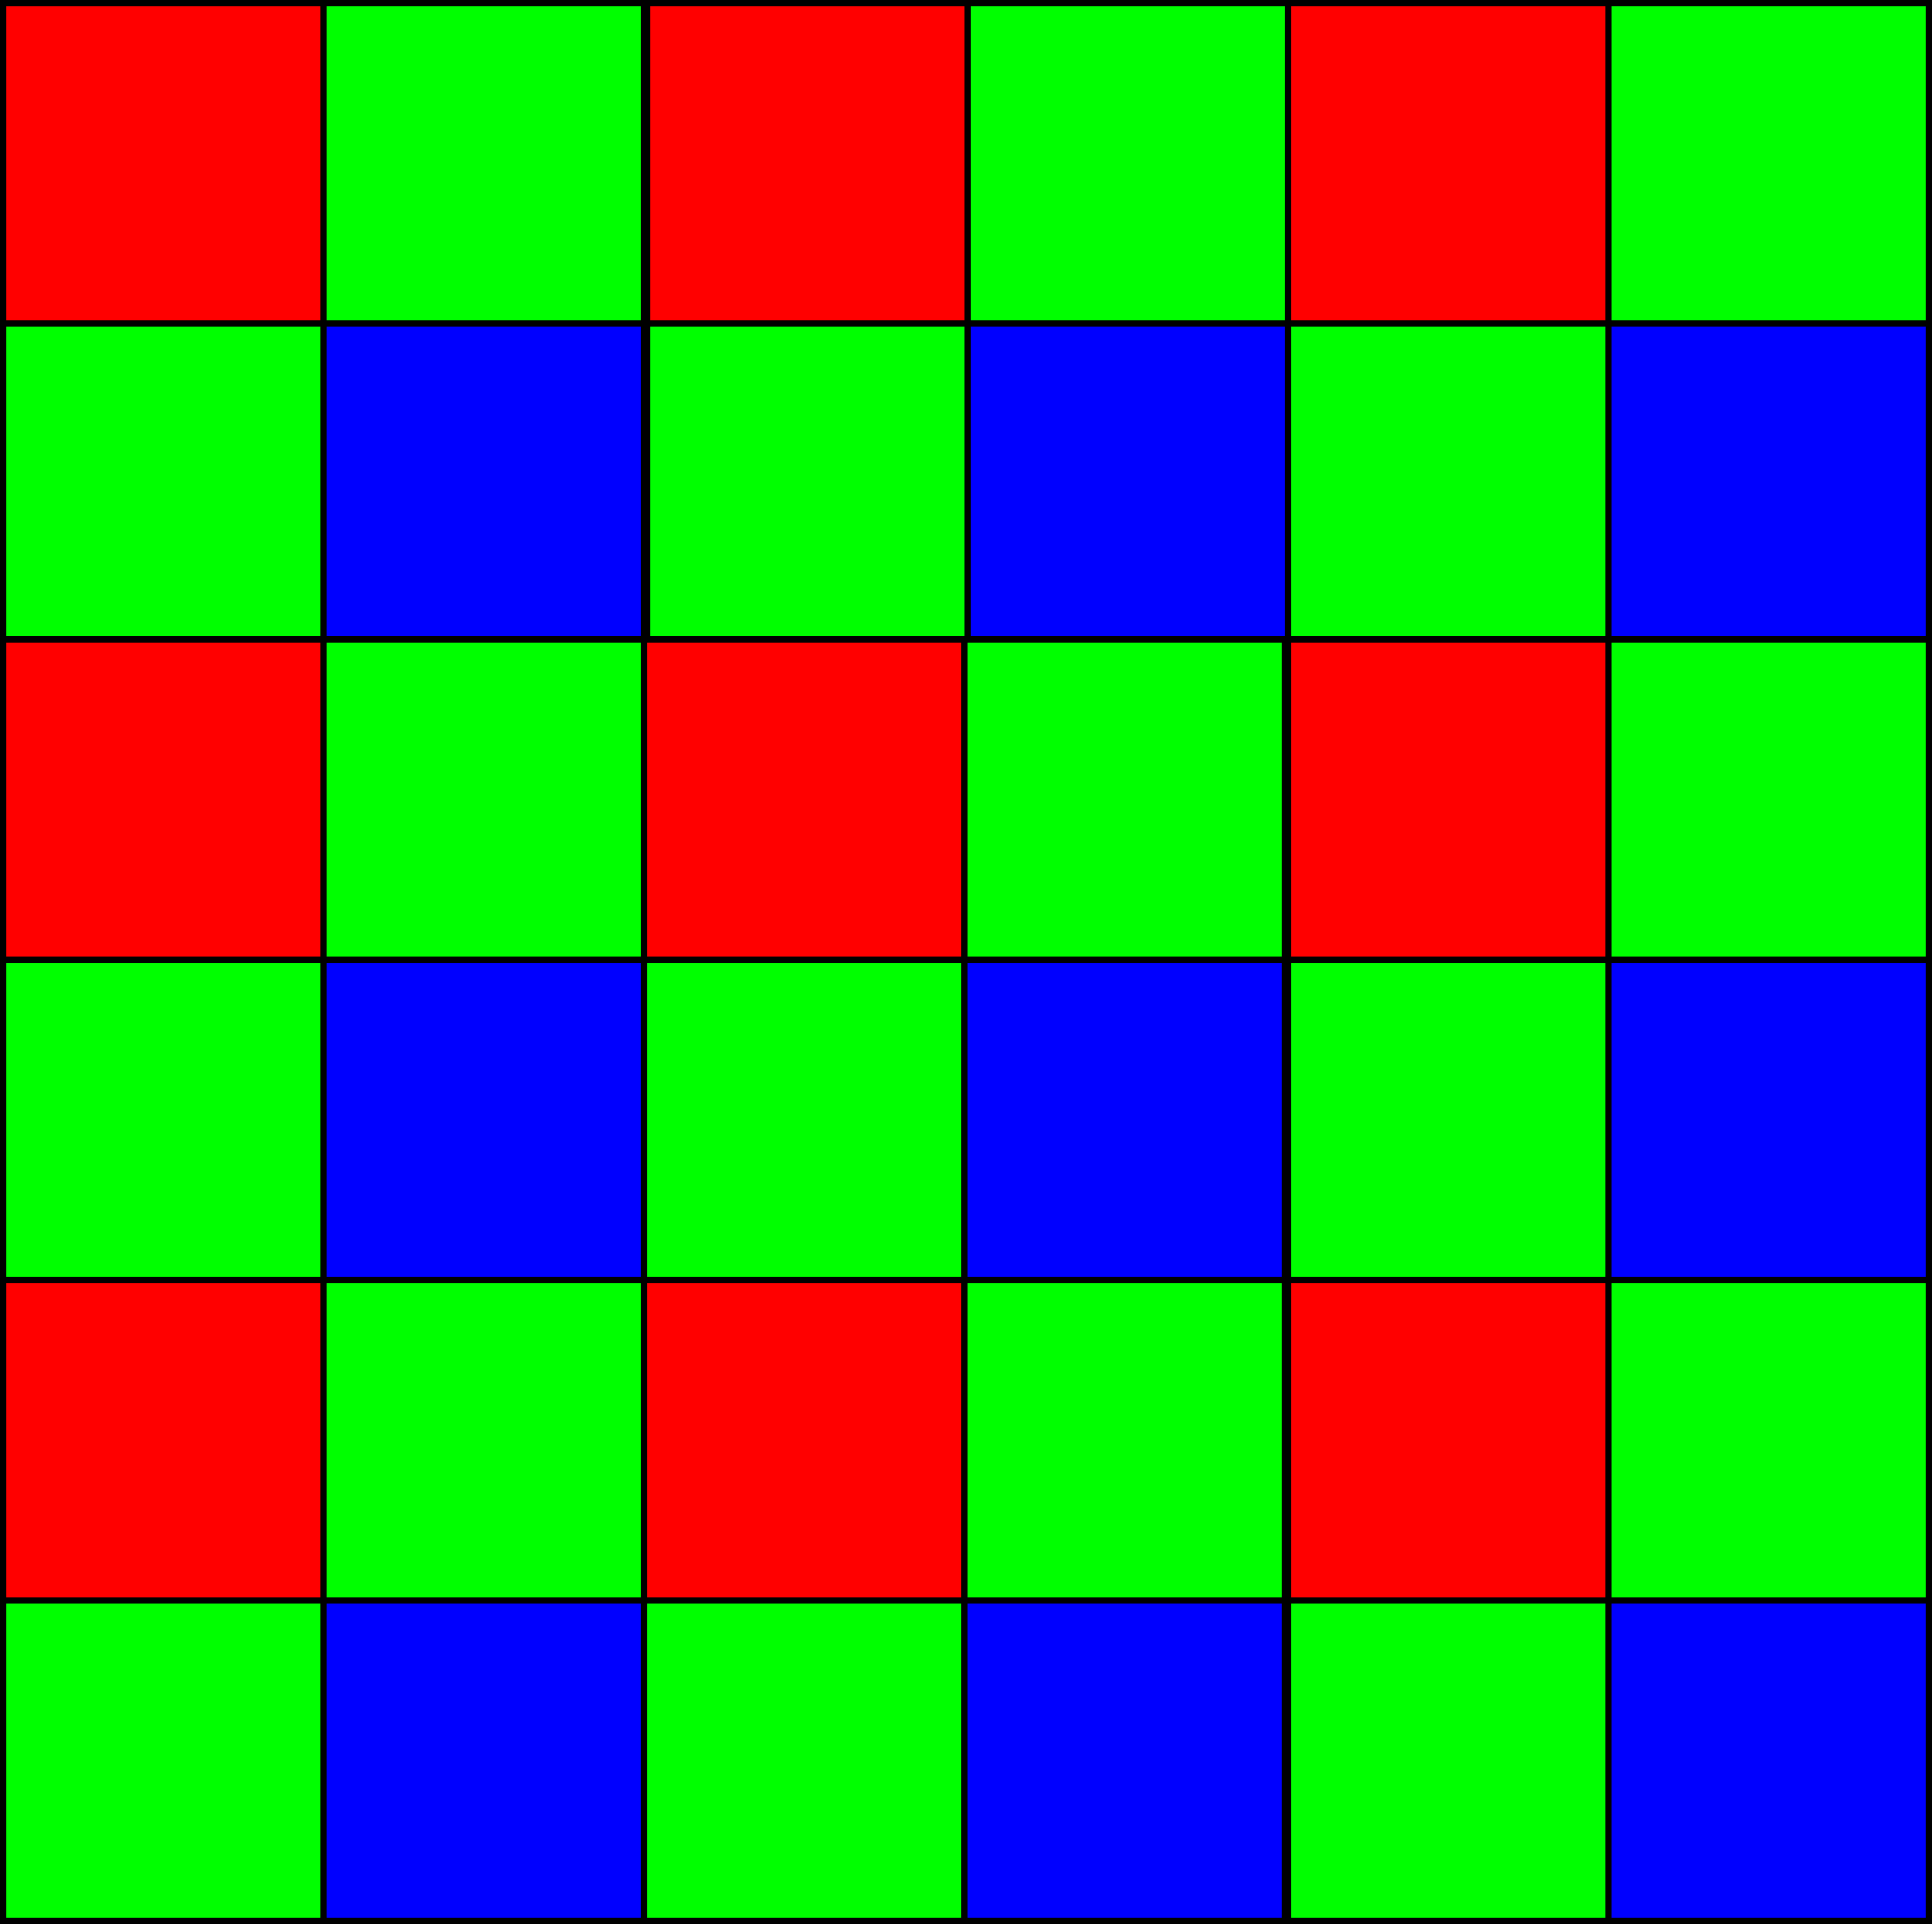
\includegraphics[width=0.3\textwidth]{figures/debayer/bayer_pattern.pdf}
    \caption{RGGB bayer pattern\cite{CommonsBayerPattern2020}}
\end{figure}

\begin{figure}[tb]
    \centering
    \begin{tabular}[b]{ccc}
        \subcaptionbox{RGGB bayer pattern}{
            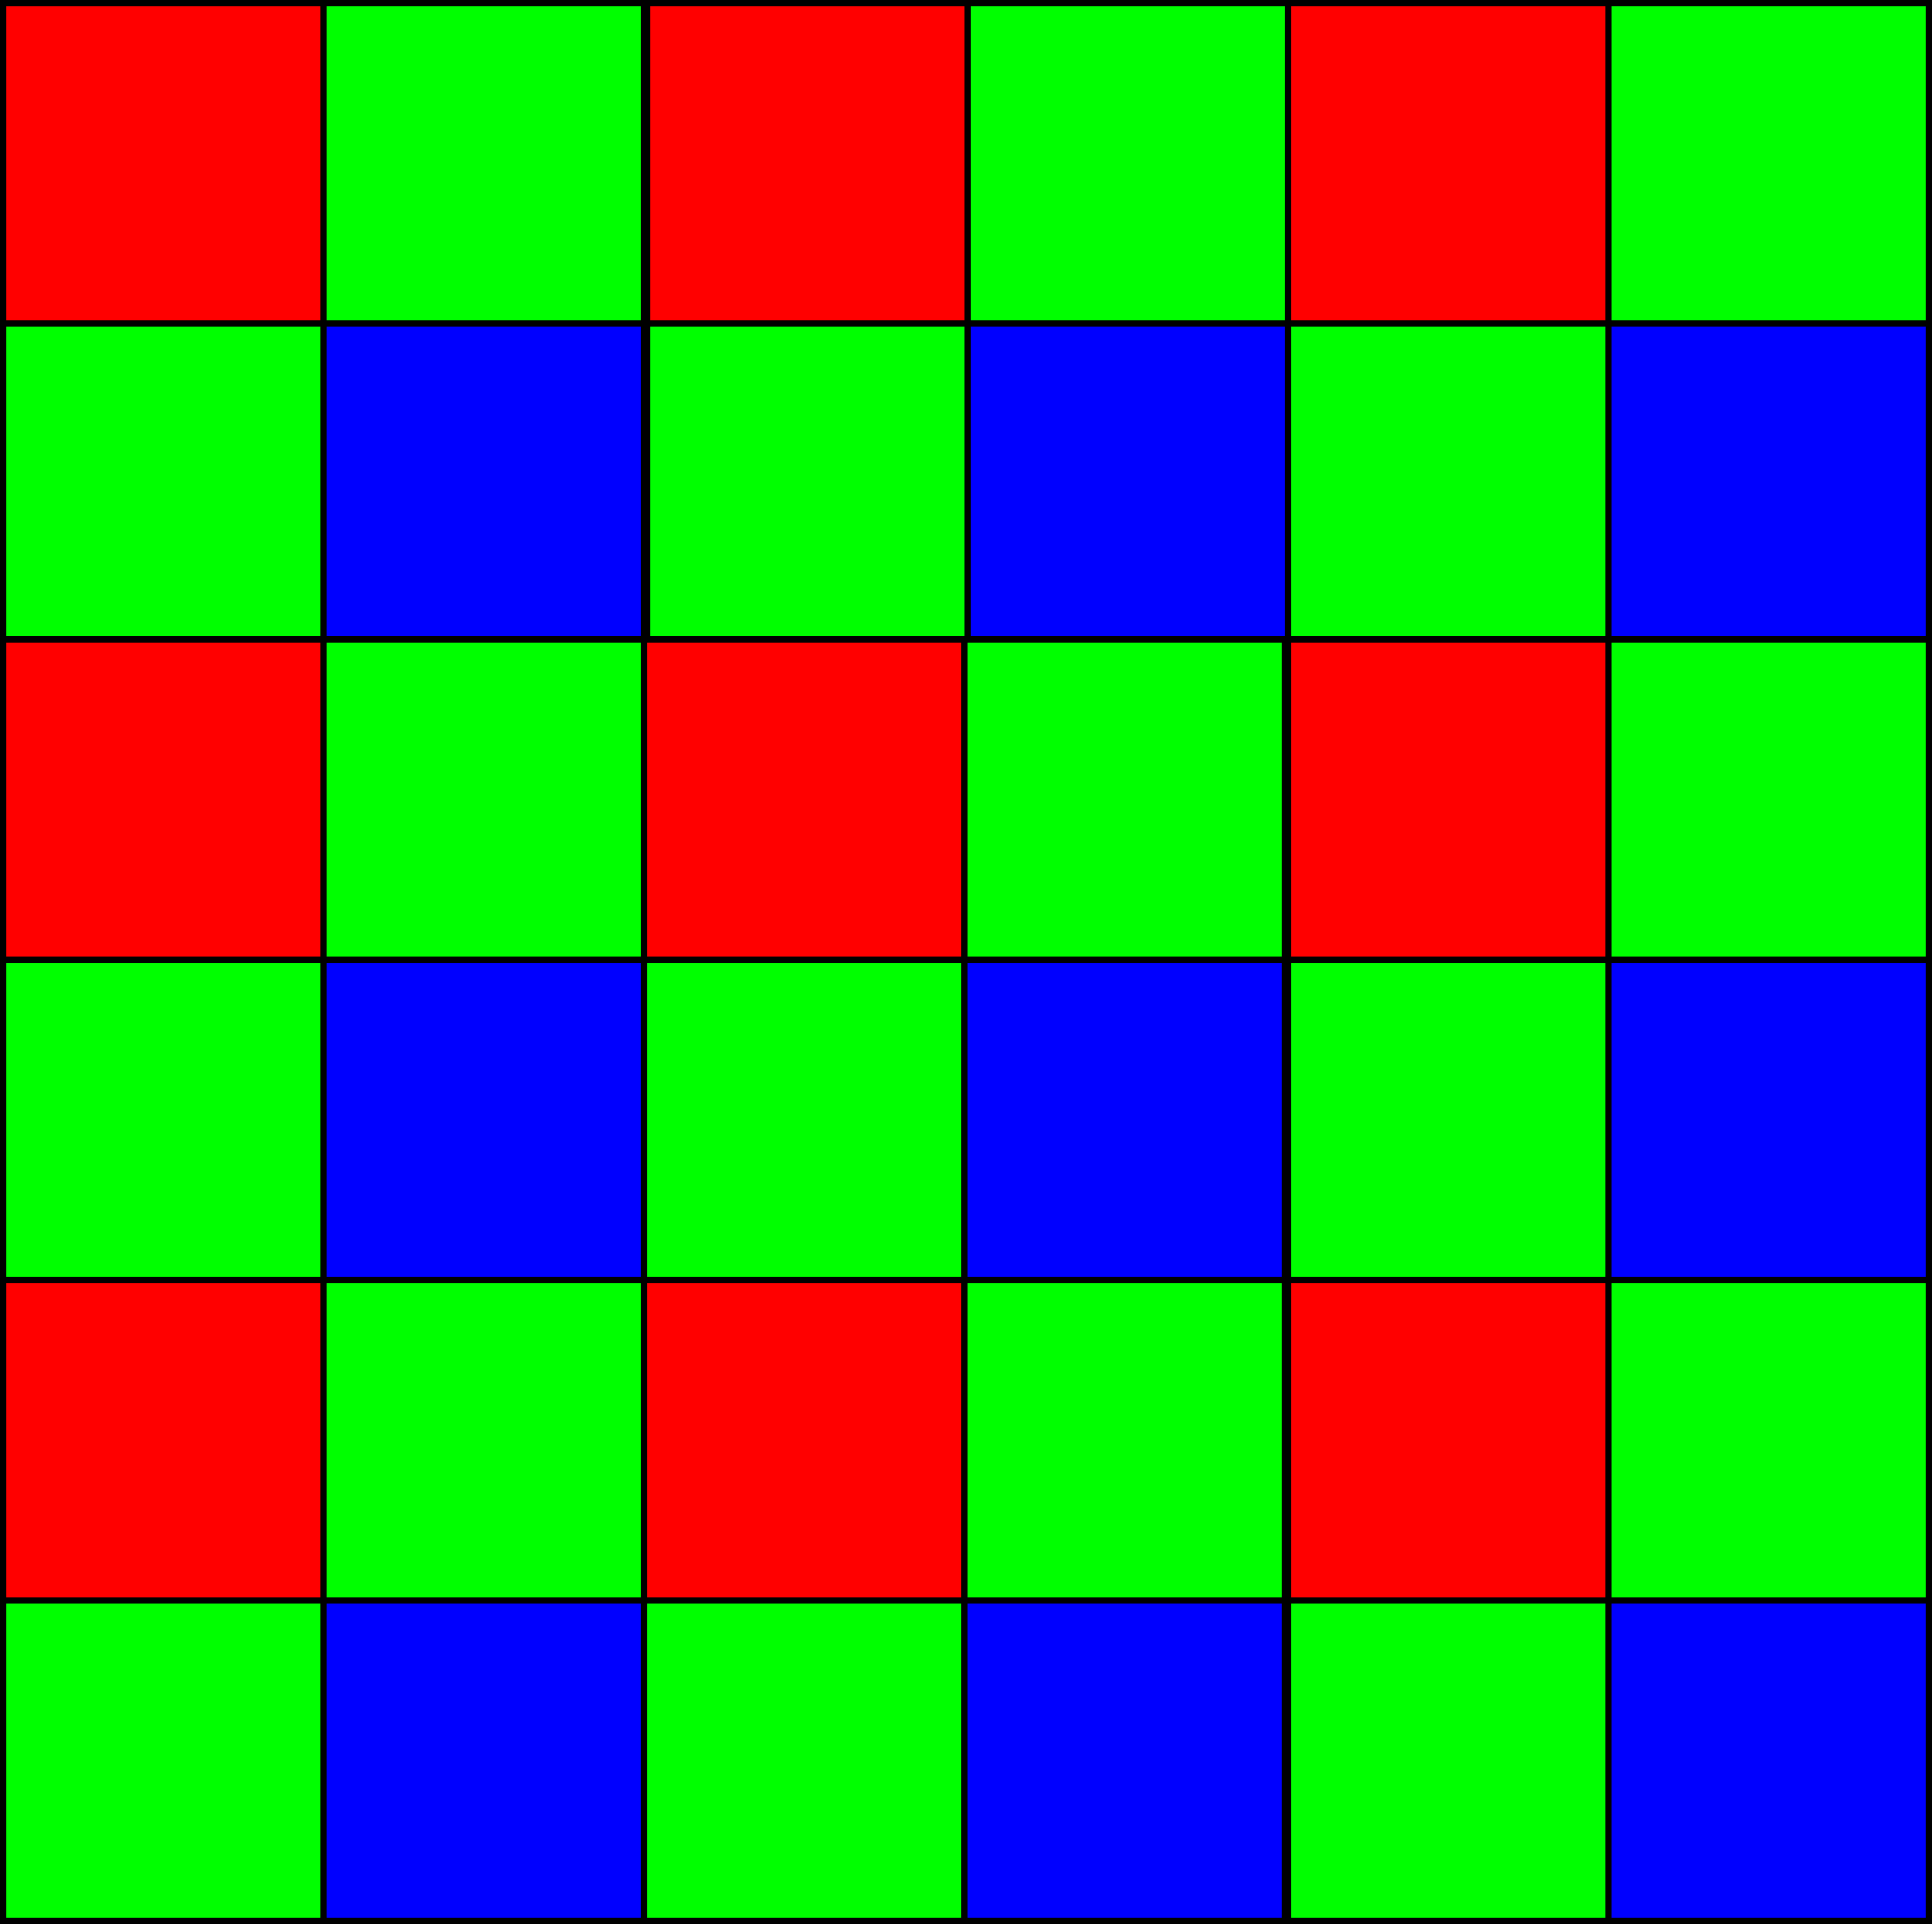
\includegraphics[width=0.25\textwidth]{figures/debayer/bayer_pattern.pdf}
        } &
        \subcaptionbox{Green at red}{
            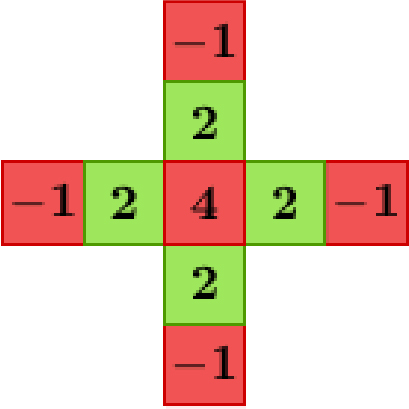
\includegraphics[width=0.25\textwidth]{figures/debayer/g_at_r.jpg}
        } &
        \subcaptionbox{Green at red}{
            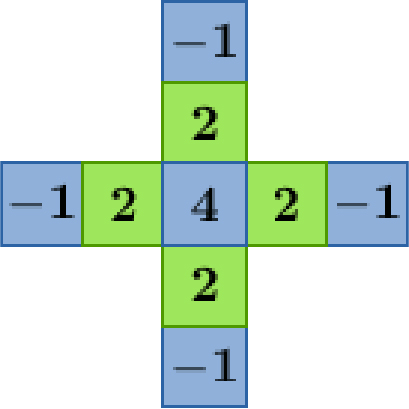
\includegraphics[width=0.25\textwidth]{figures/debayer/g_at_b.jpg}
        }
        \\
        \subcaptionbox{Red at green, red row}{
            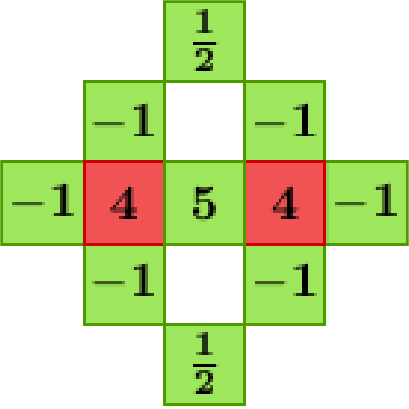
\includegraphics[width=0.25\textwidth]{figures/debayer/r_at_g_rr.jpg}
        } &
        \subcaptionbox{Red at green, blue row}{
            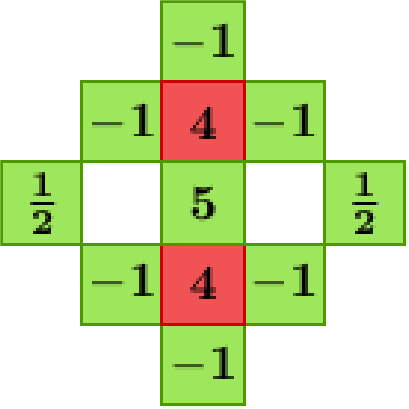
\includegraphics[width=0.25\textwidth]{figures/debayer/r_at_g_br.jpg}
        } &
        \subcaptionbox{Red at blue}{
            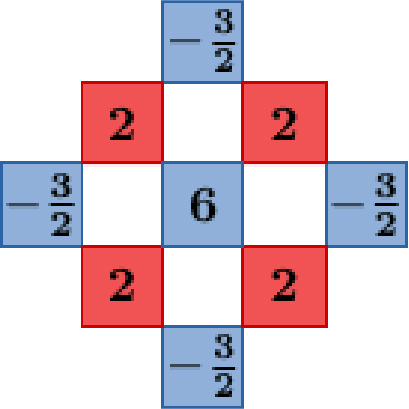
\includegraphics[width=0.25\textwidth]{figures/debayer/r_at_b.jpg}
        }
        \\
        \subcaptionbox{Blue at green, red row}{
            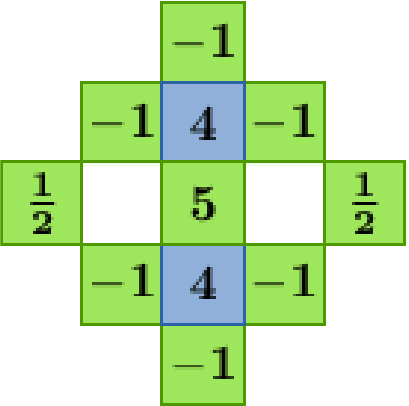
\includegraphics[width=0.25\textwidth]{figures/debayer/b_at_g_rr.jpg}
        } &
        \subcaptionbox{Blue at green, blue row}{
            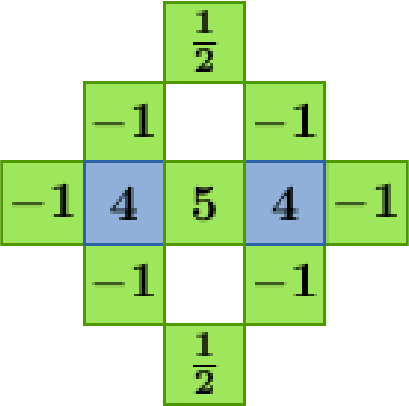
\includegraphics[width=0.25\textwidth]{figures/debayer/b_at_g_br.jpg}
        } &
        \subcaptionbox{Blue at red}{
            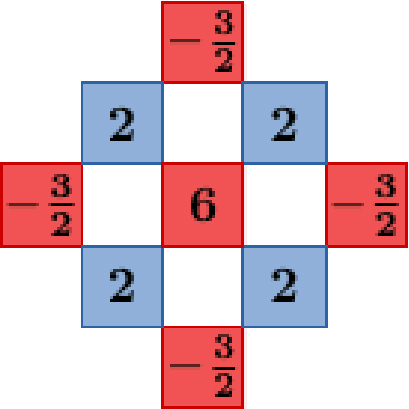
\includegraphics[width=0.25\textwidth]{figures/debayer/b_at_r.jpg}
        }
    \end{tabular}
    \caption{Coefficient values used by Malvar-He-Cutler scaled by 8 \cite{getreuerMalvarHeCutlerLinearImage2011}\cite{CommonsBayerPattern2020}}
    \label{fig:debayer:malvar_filters}
\end{figure}